% fig_adaptive_characteristic.tex
% Threshold characteristic: I_thresh vs I_rest for fixed and adaptive (k=0.10,0.15,0.20)
% Also shows CT error current: ε_CT × I_rest
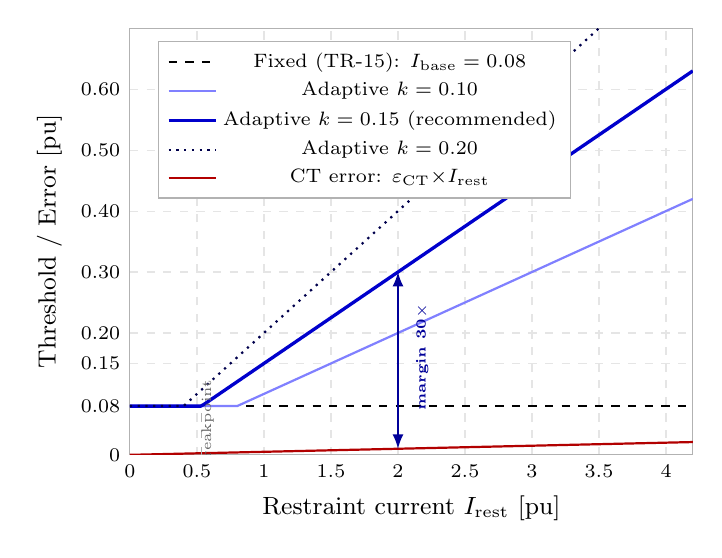
\begin{tikzpicture}
\begin{axis}[
  name        = charax,
  width       = 0.72\textwidth,
  height      = 7.0cm,
  xlabel      = {Restraint current $I_{\rm rest}$ [pu]},
  ylabel      = {Threshold / Error [pu]},
  xlabel style= {font=\small},
  ylabel style= {font=\small},
  xmin=0, xmax=4.2,
  ymin=0, ymax=0.70,
  xtick       = {0,0.5,1,1.5,2,2.5,3,3.5,4},
  ytick       = {0,0.08,0.15,0.20,0.30,0.40,0.50,0.60},
  yticklabels = {0,0.08,0.15,0.20,0.30,0.40,0.50,0.60},
  xticklabel style={font=\scriptsize},
  yticklabel style={font=\scriptsize},
  legend style={at={(0.05,0.97)}, anchor=north west,
                font=\scriptsize, draw=gray!60, fill=white},
  legend columns=1,
  grid         = major,
  grid style   = {gray!20, dashed},
  tick style   = {draw=none},
  axis line style={gray!60},
]

% ---- Fixed threshold (TR-15) -----------------------------------------------
\addplot[black, thick, dashed, domain=0:4.2, samples=2]
  {0.08};
\addlegendentry{Fixed (TR-15): $I_{\rm base}=0.08$}

% ---- Adaptive k=0.10 --------------------------------------------------------
\addplot[blue!50, thick, domain=0:4.2, samples=200]
  {max(0.08, 0.10*x)};
\addlegendentry{Adaptive $k=0.10$}

% ---- Adaptive k=0.15 (recommended) -----------------------------------------
\addplot[blue!80!black, very thick, domain=0:4.2, samples=200]
  {max(0.08, 0.15*x)};
\addlegendentry{Adaptive $k=0.15$ (recommended)}

% ---- Adaptive k=0.20 --------------------------------------------------------
\addplot[blue!30!black, thick, dotted, domain=0:4.2, samples=200]
  {max(0.08, 0.20*x)};
\addlegendentry{Adaptive $k=0.20$}

% ---- CT mismatch error (ε_CT=0.005) ----------------------------------------
\addplot[red!70!black, thick, domain=0:4.2, samples=2]
  {0.005*x};
\addlegendentry{CT error: $\varepsilon_{\rm CT}{\times}I_{\rm rest}$}

% ---- Breakpoint annotation (k=0.15 breakpoint at I_rest=0.533) -------------
\draw[gray!60, dashed, thin]
  (axis cs:0.533, 0) -- (axis cs:0.533, 0.08);
\node[font=\tiny, gray!80!black, rotate=90] at (axis cs:0.58, 0.05)
  {breakpoint};

% ---- Margin annotation at I_rest=2 -----------------------------------------
\draw[{latex}-{latex}, blue!60!black, thick]
  (axis cs:2.0, 0.01) -- (axis cs:2.0, 0.30);
\node[font=\tiny\bfseries, blue!60!black, rotate=90]
  at (axis cs:2.18, 0.16) {margin 30$\times$};

\end{axis}
\end{tikzpicture}
